\documentclass{article}

\usepackage{fancyhdr}
\usepackage{extramarks}
\usepackage{amsmath}
\usepackage{amssymb}
\usepackage{amsthm}
\usepackage{amsfonts}
\usepackage{tikz}
\usepackage[plain]{algorithm}
\usepackage{algpseudocode}
\usepackage{graphicx}
\usepackage{forest}
\usepackage{pdfpages}
\usepackage{catchfile}
\usepackage{hyperref}

\topmargin=-0.45in
\evensidemargin=0in
\oddsidemargin=0in
\textwidth=6.5in
\textheight=9.0in
\headsep=0.25in


\linespread{1.1}

\pagestyle{fancy}

\lhead{Joel Ho Eng Kiat A0200385N}
\chead{CS3219}
\rhead{Task B}
\lfoot{\lastxmark}
\cfoot{\thepage}

\begin{document}
    Link to GitHub repo \href{https://github.com/JoelHo/cs3219-assignments/tree/master/task_b}{https://github.com/JoelHo/cs3219-assignments/tree/master/task\_b}\\

    Install dependencies:

    \texttt{python3 -m venv venv}

    \texttt{source venv/bin/activate}

    \texttt{pip install -r requirements.txt}\\

    Init db:

    \texttt{python3 init\_db.py}\\

    Run app:

    \texttt{python3 main.py}\\

    \section*{B1}
    \subsection*{GET}

    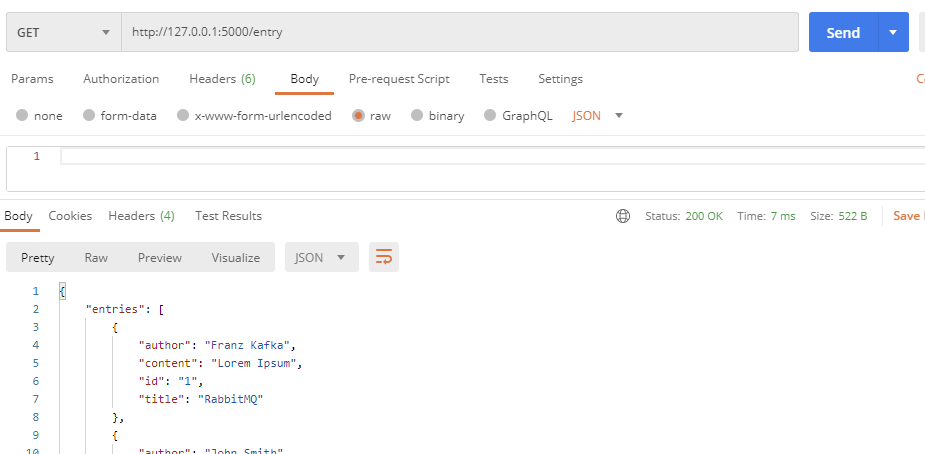
\includegraphics[width=\textwidth]{img/get.png}\\

    \subsection*{POST}

    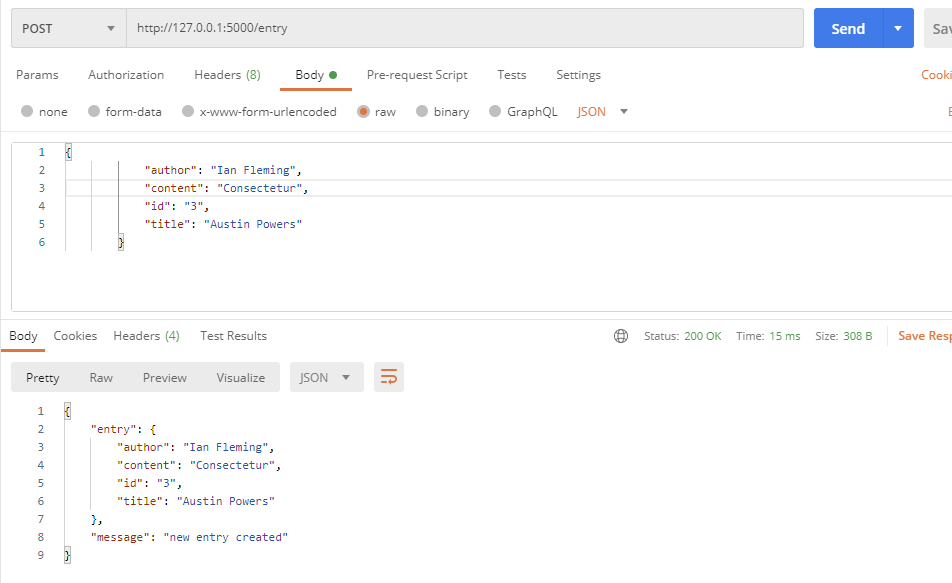
\includegraphics[width=\textwidth]{img/post.png}\\


    \subsection*{PUT}

    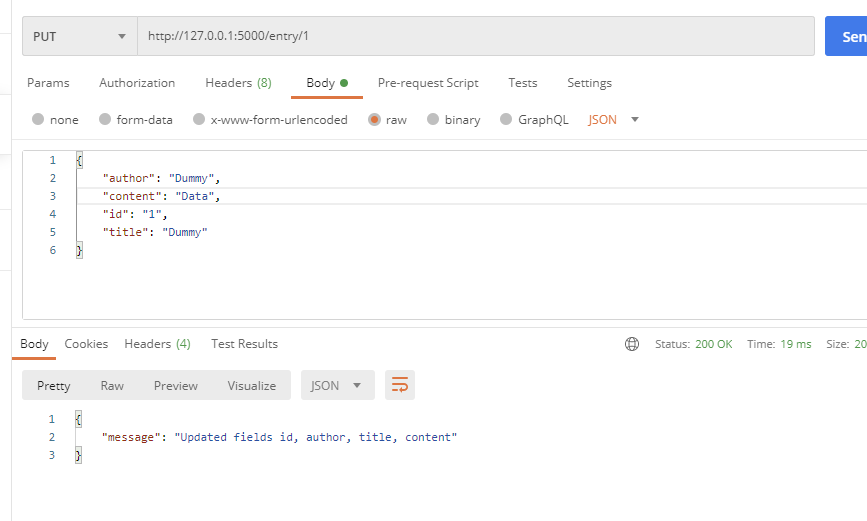
\includegraphics[width=\textwidth]{img/put.png}\\

    After PUT:

    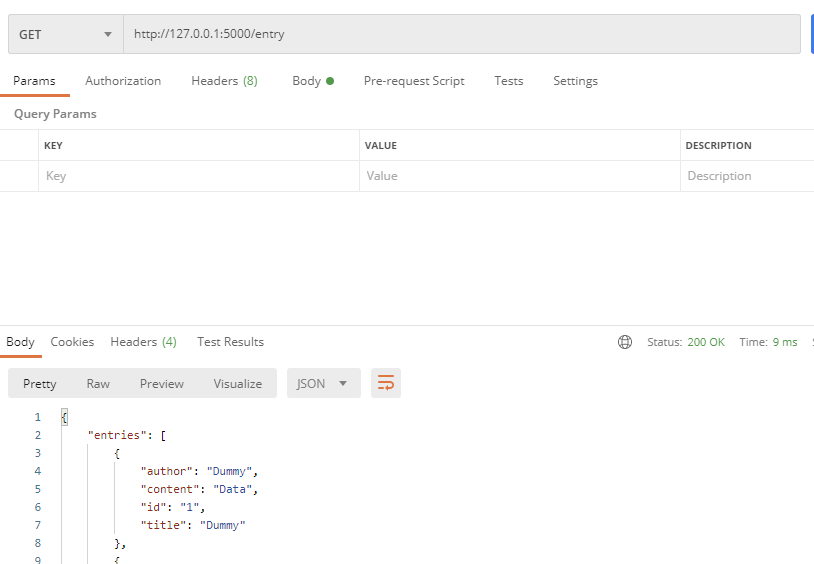
\includegraphics[width=\textwidth]{img/afterput.png}\\

    \subsection*{DELETE}

    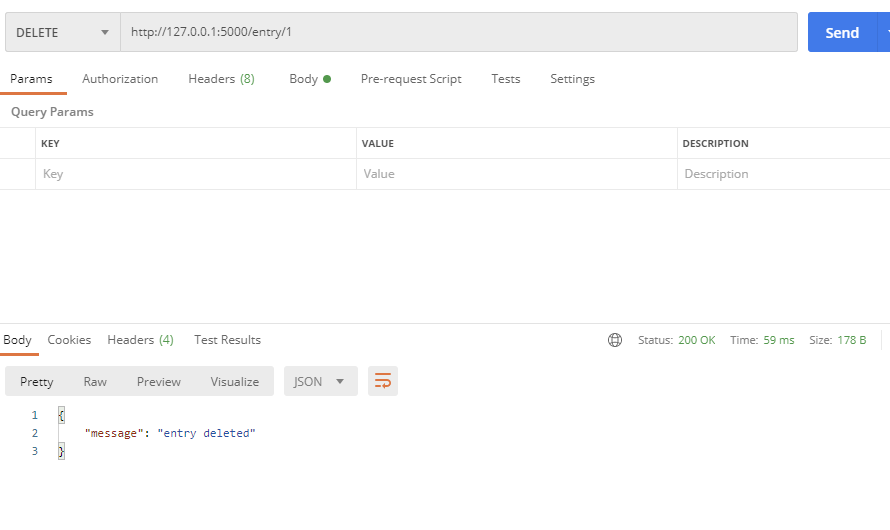
\includegraphics[width=\textwidth]{img/delete.png}\\

    \subsection*{Resilency}

    Deleting a non existent entry:

    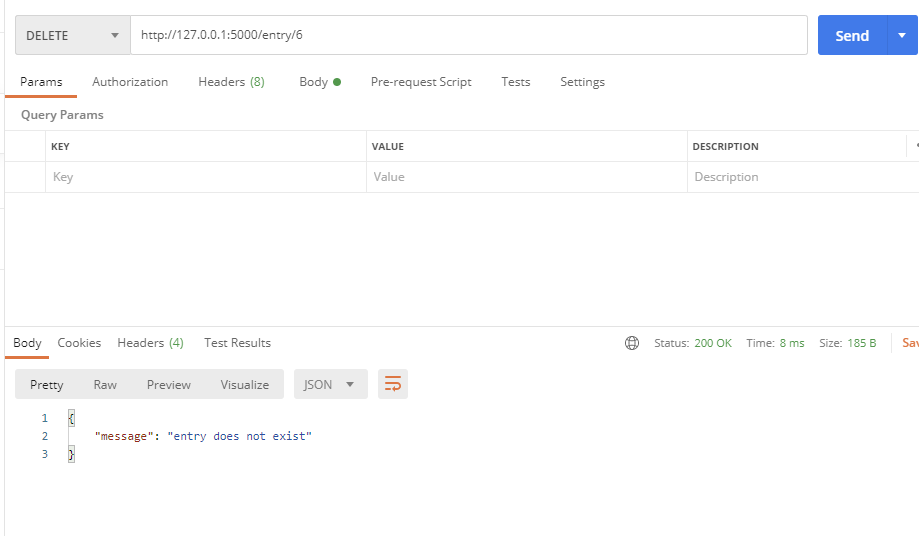
\includegraphics[width=\textwidth]{img/deleteOutRange.png}\\

    Missing field in POST:

    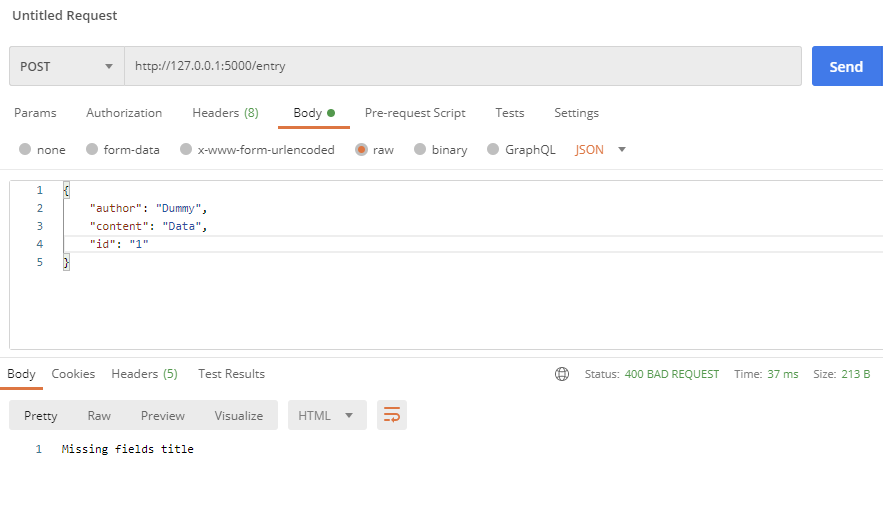
\includegraphics[width=\textwidth]{img/missingField.png}\\

    Empty PUT:

    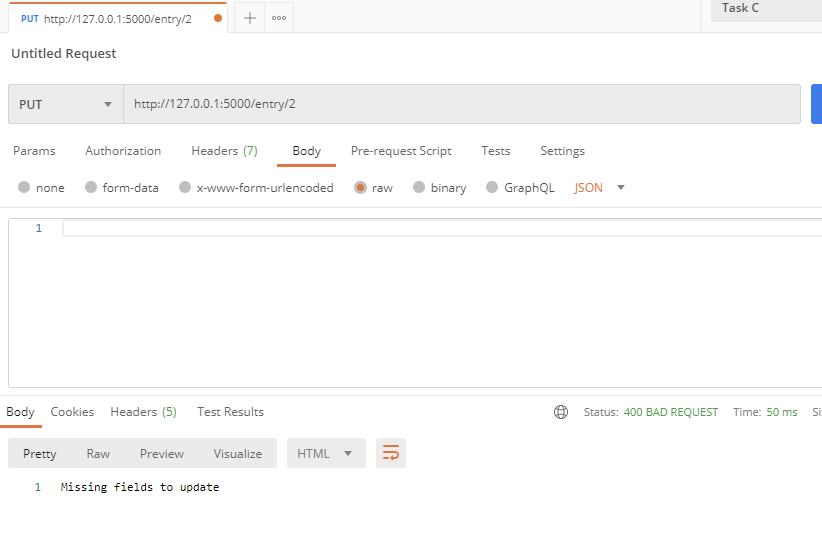
\includegraphics[width=\textwidth]{img/missingPut.png}\\






\end{document}
